\section{Exact checks and reproducible examples}\label{sec:validation}

The universal statements above are proved analytically. The accompanying Python program
\texttt{code/verify\_symplectic.py} supplies independent finite checks using rational arithmetic;
the numerical calculations are not premises of the proof. It implements the finite embedding
counts, Gaussian moment inversion, the independent-entry rank formula, the residual nullity
law, and the exact joint law. It then compares those formulas with direct enumeration of
Gram fibres. The enumeration does not use the embedding formula or the moment identities.

The direct checks enumerate $209{,}846$ matrices across nine configurations over
$\mathbb F_2,\mathbb F_3,\mathbb F_4,\mathbb F_5$, including rectangular $4\times2$ and
$6\times2$ blocks and square $4\times4$ blocks. Arithmetic in $\mathbb F_4$ uses
$\mathbb F_2[x]/(x^2+x+1)$, not the ring $\mathbb Z/4\mathbb Z$. All exact comparisons pass.
The broader calculation checks $290$ parameter triples over field sizes $2,3,4,5,7$, with
$2\le b\le24$ and several gaps up to $a=3b+2$. It includes $84$ exact joint-law calculations.

For selected binary examples, the distances are:
\begin{center}
\begin{tabular}{rrcc}
\toprule
$a$ & $b$ & Full matrix distance & Rank distance\\
\midrule
10&8&$0.1305891625$&$7.513114553\cdot10^{-4}$\\
18&16&$0.1306341717$&$2.937693211\cdot10^{-6}$\\
26&24&$0.1306343460$&$1.147540771\cdot10^{-8}$\\
48&24&$0.1306343462$&$3.552713255\cdot10^{-15}$\\
\bottomrule
\end{tabular}
\end{center}
These values are rounded from exact rational probabilities. For example, for $q=2$,
$(a,b)=(4,4)$ the full distance is $6767/52224$, the rank distance is $1087/52224$,
and the joint-versus-product distance is $0.0584037601947784423828125$ exactly.

\begin{figure}[htbp]
\centering
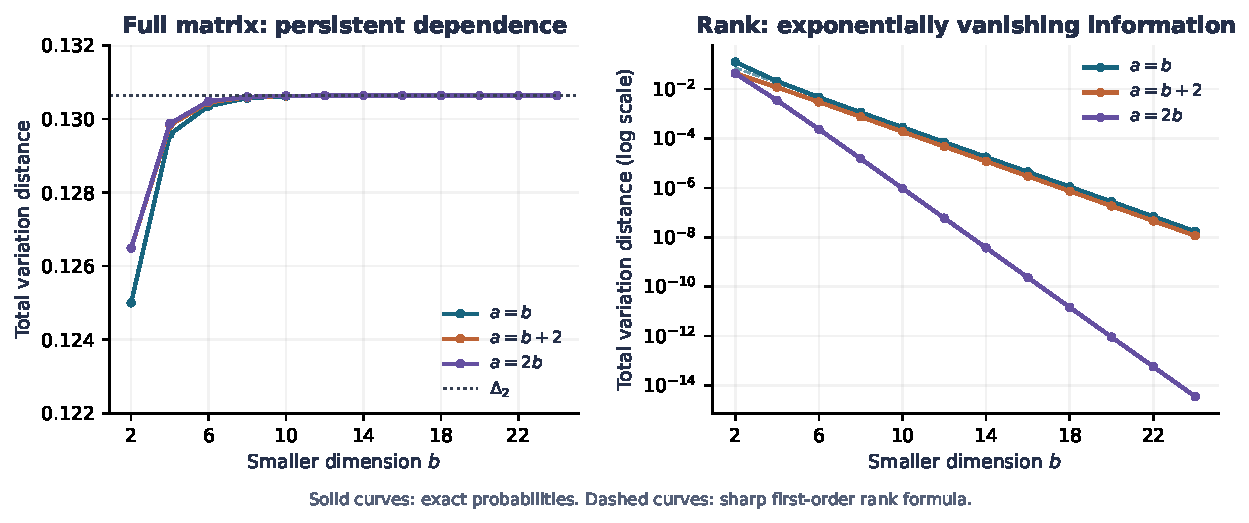
\includegraphics[width=\textwidth]{figures/symplectic_separation.pdf}
\caption{Uniform separation across shapes over $\mathbb F_2$. The complete matrix retains
a fixed testing advantage, while rank alone loses information exponentially in the larger dimension.
The dashed curves on the right are the proved first-order formula, not fitted regressions.}
\label{fig:separation}
\end{figure}

The data files retain the exact-enumeration receipts, high-precision comparison values, and
scaled remainders. Decimal evaluations use $150$ digits and $160$ factors of the infinite products.
The observed scaled remainders are evidence of agreement with the formulas; their finite maxima
are not asserted to be universal bounds. Both the main paper and the companion filter note
contain human-readable proofs. This packet contains no newly kernel-checked Lean formalization.
